\documentclass{article}

% ------------------------------------ %
%             Document Info            %
% ------------------------------------ %

\usepackage{../../../LaTeX-Preamables/Assign}

\begin{document}
\newcommand{\documentcourse}{MATH1851}
\newcommand{\documentnumber}{3}

% ------------------------------------ %
%                Header                %
% ------------------------------------ %

\begin{minipage}{0.07\textwidth}
    
\includegraphics[width=\linewidth]{../../../LaTeX-Preamables/LaTeX-Templates/HKULOGO256.png}
\end{minipage}
\hspace{0.02\textwidth}
\begin{minipage}{0.55\textwidth}
    \documentcourse

    Assignment \documentnumber

    SID: 3036268218
\end{minipage}
\begin{minipage}{0.35\textwidth}
    \begin{flushright}
        Jax

        \jobname.pdf

        \today
    \end{flushright}
\end{minipage}

\vspace{0.5cm}

\hrule

% ------------------------------------ %
%                Content               %
% ------------------------------------ %

\section*{Question 1}
\begin{align*}
    J & =\int_0^1\sqrt{1-x^4}\:dx \\K&=\int_0^1\sqrt{1+x^4}\:dx\\L&=\int_0^1\sqrt{1-x^8}\:dx
\end{align*}
Order the definite integrals above and 1 from smallest to largest. Justify!
\\
The order is $J < L < 1 < K$.
\begin{itemize}
    \item $K > 1$ because at this interval, $\sqrt{1+x^4} \in (1,\sqrt{2})$, so the area must exceed 1.
    \item $1 > L, J$ because at this interval, $\sqrt{1-x^n} \in (0,1)$, so the area must be less than 1.
    \item $L$ and $J$ is a decreasing function as $\sqrt{1-x^n}' = -\frac{nx^{n-1}}{2\sqrt{1-x^n}} < 0$. We can simply take a point in the interval and compare the values of the functions to see that $L > J$: $\sqrt{1-0.5^8} =  > \sqrt{1-0.5^4}$. Therefore, the area of $n=8$ for $\sqrt{1-x^n}$ is greater than $n=4$, so $L > J$.
\end{itemize}

\section*{Question 2}
Make a substitution and use the method of partial fractions to evaluate
\[\int\frac{\cos x}{\sin^2x+\sin x}dx.\]
\begin{align*}
    \int\frac{\cos x}{\sin^2x+\sin x}dx & =\int\frac{\cos x}{\sin x(\sin x+1)}dx \\
    \text{Let }u=\sin x \rightarrow du  & =\cos x\:dx                            \\
    \int\frac{1}{u(u+1)}du              & =\int(\frac{1}{u}-\frac{1}{u+1})du     \\
                                        & =\ln|u|-\ln|u+1|+c                     \\
                                        & =\ln|\sin x|-\ln|\sin x+1|+c
\end{align*}

\section*{Question 3}
Complete the square and use trigonometric substitution to evaluate
\[\int\frac{dt}{\sqrt{t^2-6t+13}}.\]
\begin{align*}
    \int\frac{1}{\sqrt{t^2-6t+13}}\:dt                        & =\int\frac{1}{\sqrt{(t-3)^2+4}}\:dt                    \\
                                                              & =\int\frac{1}{2\sqrt{(\frac{t-3}{2})^2+1}}\:dt         \\
    \text{Let }\frac{t-3}{2}=\tan\theta \rightarrow dt        & =2\sec^2\theta d\theta                                 \\
    \int\frac{2\sec^2\theta}{2\sqrt{\tan^2\theta+1}}\:d\theta & =\int\frac{\sec^2\theta}{\sqrt{\sec^2\theta}}\:d\theta \\
                                                              & =\int\sec\theta\:d\theta                               \\
                                                              & =\ln|\sec\theta+\tan\theta|+c                          \\
    \sec\theta = \sqrt{1+\tan^2\theta}\rightarrow             & =\ln|\frac{t-3}{2}+\sqrt{(\frac{t-3}{2})^2+1}|+c       \\
                                                              & = \ln|t-3+\sqrt{(t-3)^2+4}|-\ln2+c                     \\
                                                              & = \ln|t-3+\sqrt{(t-3)^2+4}|+c
\end{align*}
\section*{Question 4}
Use Integration by Parts to prove the reduction formula
\[I_n=\int x^n\cos x\:dx=x^n\sin x+nx^{n-1}\cos x-n(n-1)I_{n-2}.\]
\begin{align*}
    \int uv                                                        & =u\int v-\int (u'\times \int v)               \\
    \text{Let }u                                                   & =x^n\rightarrow u'=nx^{n-1}                   \\
    \text{Let }v                                                   & =\cos x\rightarrow \int v=\sin x              \\
    I_n                                                            & =x^n\sin x-\int(nx^{n-1}\sin x)\:dx           \\
    \\
    \int(nx^{n-1}\sin x)\:dx                                       & =-nx^{n-1}\cos x+n(n-1)\int x^{n-2}\cos x\:dx \\
    \because I_{n-2}          = \int x^{n-2}\cos x\:dx \rightarrow & = -nx^{n-1}\cos x+n(n-1)I_{n-2}               \\
    \\
    \therefore I_n                                                 & =x^n\sin x-(-nx^{n-1}\cos x+n(n-1)I_{n-2})    \\
                                                                   & =x^n\sin x+nx^{n-1}\cos x-n(n-1)I_{n-2}
\end{align*}
\section*{Question 5}
\subsection*{Question 5a}
Use the Quotient Rule for differentiation and the Fundamental Theorem of Calculus to find a rule to integrate quotients.
\begin{align*}
    (\frac{a}{b})'   & =\frac{ba'-ab'}{b^2}                \\
    (\frac{a}{b})'   & = \frac{a'}{b}-\frac{ab'}{b^2}      \\
    \frac{a'}{b}     & = \frac{ab'}{b^2} + (\frac{a}{b})'  \\
    \int\frac{a'}{b} & = \int\frac{ab'}{b^2} + \frac{a}{b} \\
\end{align*}
\subsection*{Question 5b}
Use your rule to integrate quotients to evaluate the following, and verify the correctness
\[\int\frac{\sin{(x^{-\frac{1}{2}})}}{x^2}dx\]
\begin{align*}
    \text{Note that we are looking for }                                        & a'\text{ consisting }\sin(x^{-\frac{1}{2}}):                                                                     \\
    \text{Let }a                                                                & = 2\cos(x^{-\frac{1}{2}}) \rightarrow a' =x^{-\frac{3}{2}}\sin(x^{-\frac{1}{2}})                                 \\
    \text{Let }b                                                                & = x^{\frac{1}{2}} \rightarrow b' = \frac{1}{2}x^{-\frac{1}{2}}                                                   \\
    \\
    \int\frac{a'}{b}                                                            & = \int\frac{ab'}{b^2} + \frac{a}{b}                                                                              \\
    \int\frac{\sin{(x^{-\frac{1}{2}})}}{x^{(\frac{1}{2}+\frac{3}{2})}}\:dx      & = \int\frac{2\cos(x^{-\frac{1}{2}})\frac{1}{2}x^{-\frac{1}{2}}}{x}\:dx + \frac{2\cos(x^{-\frac{1}{2}})}{x^{1/2}} \\
                                                                                & = \int x^{-\frac{3}{2}}\cos(x^{-\frac{1}{2}})\:dx + 2\frac{\cos(x^{-1/2})}{x^{1/2}}                              \\
    \because (2\cos(x^{-\frac{1}{2}}))' =x^{-\frac{3}{2}}\sin(x^{-\frac{1}{2}}) & \rightarrow-2\sin(x^{-\frac{1}{2}}) = \int x^{-\frac{3}{2}}\cos(x^{-\frac{1}{2}})\:dx                            \\
    \therefore                                                                  & = -2\sin(x^{-\frac{1}{2}}) + 2\frac{\cos(x^{-\frac{1}{2}})}{x^{\frac{1}{2}}} + c                                 \\
\end{align*}
Verification:
\begin{align*}
    {Let }u                                    & = x^{-\frac{1}{2}} \rightarrow du = -\frac{1}{2}x^{-\frac{3}{2}}\:dx               \\
    \int\frac{\sin{(x^{-\frac{1}{2}})}}{x^2}dx & = \int x^{-\frac{3}{2}}x^{-\frac{1}{2}}(-\frac{1}{2})(-2)\sin x^{-\frac{1}{2}}\:dx \\
                                               & = \int -2u\sin u\:du                                                               \\
                                               & = -2(-u\cos u-\int -\cos u\:du) + c                                                \\
                                               & = 2x^{-\frac{1}{2}}\cos x^{-\frac{1}{2}}-2\sin x^{-\frac{1}{2}}+c                  \\
                                               & = -2\sin(x^{-\frac{1}{2}}) + 2\frac{\cos(x^{-1/2})}{x^{1/2}} + c
\end{align*}
\section*{Question 6}
A Bundt cake, well known for having a ringed shape, is formed by revolving around the y-axis the region bounded by the graph of $y = sin(x^2 -1)$ and the x-axis over the interval $1 \le x \le \sqrt{1+\pi}$. Find the volume of the cake
% \begin{align*}
%     y                                                              & = \sin(x^2-1)                                                  \\
%     R(y)                                                           & = \sqrt{\sin^{-1}y+1}                                          \\
%     \\
%     \text{For the section interested, the min/max is 0/1. So for } & R(y) \text{ the corresponding interval is (0,1)}               \\
%     V                                                              & = \pi\int_{0}^{1}R^2(y)\:dy                                    \\
%                                                                    & = \pi\int_{0}^{1}(\sin^{-1}y+1)\:dy                            \\
%                                                                    & = \pi[y\sin^{-1}y-\int\frac{y}{\sqrt{1-y^2}}\:dy + y]_{0}^{1}  \\
%     (\sqrt{1-y^2})' = -\frac{y}{\sqrt{1-y^2}}\rightarrow           & = \pi[y\sin^{-1}y+\sqrt{1-y^2} + y]_{0}^{1}                    \\
%                                                                    & = \pi[1\sin^{-1}1+\sqrt{1-1} + 1 - 0\sin^{-1}0-\sqrt{1-0} - 0] \\
%                                                                    & = \pi[1\frac{\pi}{2}+1]                                        \\
%                                                                    & = \frac{\pi^2}{2}+ \pi
% \end{align*}
\begin{align*}
    V                                 & = \pi\int_{a}^{b}2(x+r)R(x)\:dx                   \\
    r=0 \to                           & = \pi\int_{1}^{\sqrt{1+\pi}}2(x)(\sin(x^2-1))\:dx \\
    (-\cos(x^2-1))'=2x\sin(x^2-1) \to & = \pi[-\cos(x^2-1)]_{1}^{\sqrt{1+\pi}}            \\
                                      & = \pi(-\cos(1+\pi-1)+\cos(1-1))                   \\
                                      & = \pi(-\cos(\pi)+1)                               \\
                                      & = \pi(1+1)                                        \\
                                      & = 2\pi
\end{align*}

\section*{Question 7}
Find the perimeter of the shape formed by $x^{2/3}+y^{2/3}=1$:
\begin{center}
    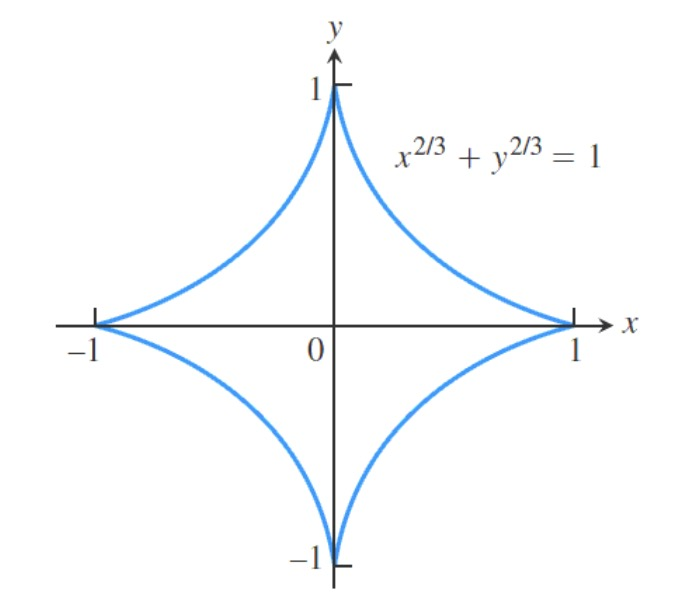
\includegraphics[width=0.2\textwidth]{A3Q7.jpg}
\end{center}
We can parametize the equation for easier calculation:
\begin{align*}
    x^{2/3}+y^{2/3}   & =1                \\
    \sin^2t + \cos^2t & = 1               \\
    x                 & =\sin^3 t         \\
    y                 & =\cos^3 t         \\
    x'                & =3\sin^2 t\cos t  \\
    y'                & =-3\cos^2 t\sin t \\
\end{align*}
To find the length of a side, we are interested in $x\in[0,1]\to t\in[0,\pi/2]$:
\begin{align*}
    L            & =\int_{0}^{\pi/2}\sqrt{x'^2+y'^2}\:d t                           \\
                 & =\int_{0}^{\pi/2}\sqrt{9\sin^4 t\cos^2 t+9\cos^4 t\sin^2 t}\:d t \\
                 & =3\int_{0}^{\pi/2}\sin t\cos t\:d t                              \\
                 & =\frac{3}{2}\int_{0}^{\pi/2}\sin 2t\:d t                         \\
                 & =\frac{3}{2}[\frac{-\cos 2t}{2}]_{0}^{\pi/2}                     \\
                 & =\frac{3}{2}[\frac{-\cos \pi}{2}+\frac{\cos 0}{2}]               \\
                 & =\frac{3}{2}                                                     \\
    \therefore P & = 4 \times \frac{3}{2} = 6
\end{align*}


\section*{Question 8}
\emph{Use the integral formula for arc length to show that the shortest distance between two points is a line:}

The arc length formula $L=\int_{a}^{b}\sqrt{1+f'^2(x)}\:dx$ is simply the submation of the distance between two points. The horizontal distance between two points is $dx$, and the vertical distance is $dy=f'(x)dx$.
Hence, the distance is given by the Pythagorean theorem, $\sqrt{1+f'^2(x)}\times dx$.

There we can see how the arc length formula is defined as the sum of the \textbf{straight-line distance between points} in the interval $[a,b]$. Therefore, the shortest distance between two points is a line.


\end{document}